
\documentclass[12pt,a4paper]{article}

\usepackage[utf8]{inputenc}
\usepackage[T1]{fontenc}
\usepackage{polski}

\usepackage{amsthm}
\usepackage{amsmath}
\usepackage{amsfonts}
\usepackage{amssymb}
\usepackage{pgfplots}
\usepackage{tikz}
\usepackage{lmodern}	%fancy font
\usepackage{textcomp}

\usepackage{indentfirst}
\usepackage{graphicx}
\usepackage{caption}
\usepackage{subcaption}
%\usepackage{siunitx}
\usepackage{here}


\setlength{\textheight}{24cm}
\setlength{\textwidth}{15.92cm}
\setlength{\footskip}{10mm}
\setlength{\oddsidemargin}{0mm}
\setlength{\evensidemargin}{0mm}
\setlength{\topmargin}{0mm}
\setlength{\headsep}{5mm}
\usepackage{tikz}
\usepackage{lmodern}	%fancy font
\usepackage{textcomp}

\usepackage{indentfirst}
\usepackage{graphicx}
\usepackage{caption}
\usepackage{subcaption}
%\usepackage{siunitx}
\usepackage{here}
\usepackage[margin=1in]{geometry}% Just for this example
\setlength{\parindent}{0pt}% Just for this example
\setlength{\textheight}{24cm}
\setlength{\textwidth}{15.92cm}
\setlength{\footskip}{10mm}
\setlength{\oddsidemargin}{0mm}
\setlength{\evensidemargin}{0mm}
\setlength{\topmargin}{0mm}


\begin{document}

\begin{table}[]
\label{my-label}
\begin{tabular}{|p{7.5cm}|p{7.5cm}|}
\hline
									           					&                           \\

\includegraphics[height=3cm]{logo}             					& \textbf{Technika cyfrowa} \\ \hline
\multicolumn{1}{|l|}{\textbf{Temat ćwiczenia}} 					& \textbf{Numer ćwiczenia}  \\
\multicolumn{1}{|l|}{Liczniki}	& 2                         \\ \hline
\multicolumn{1}{|l|}{\textbf{Wykonawca}}       & \textbf{Ocena}            \\
\multicolumn{1}{|l|}{Marcin Przewięźlikowski}          &                           \\ \hline
\end{tabular}
\end{table}

\section{Cel ćwiczenia}

Zapoznanie się z zastosowaniem przerzutników w budowaniu liczników synchronicznych oraz asynchronicznych. Zbadanie działania liczników czterobitowych.

\section{Dwójka licząca}


Dwójka licząca służy do dzielenia częstotliwości sygnału wejściowego przez 2. Uzyskano ją na dwa sposoby:

\subsection{Przerzutnik D}


Dwójka licząca służy do dzielenia częstotliwości sygnału wejściowego przez 2. Oto jej tabela prawdy:



\begin{figure}[H]
\centering
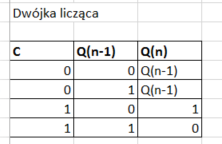
\includegraphics{img/4a_table}
\end{figure}

Uzyskano ją na dwa sposoby:

\begin{figure}[H]
\centering
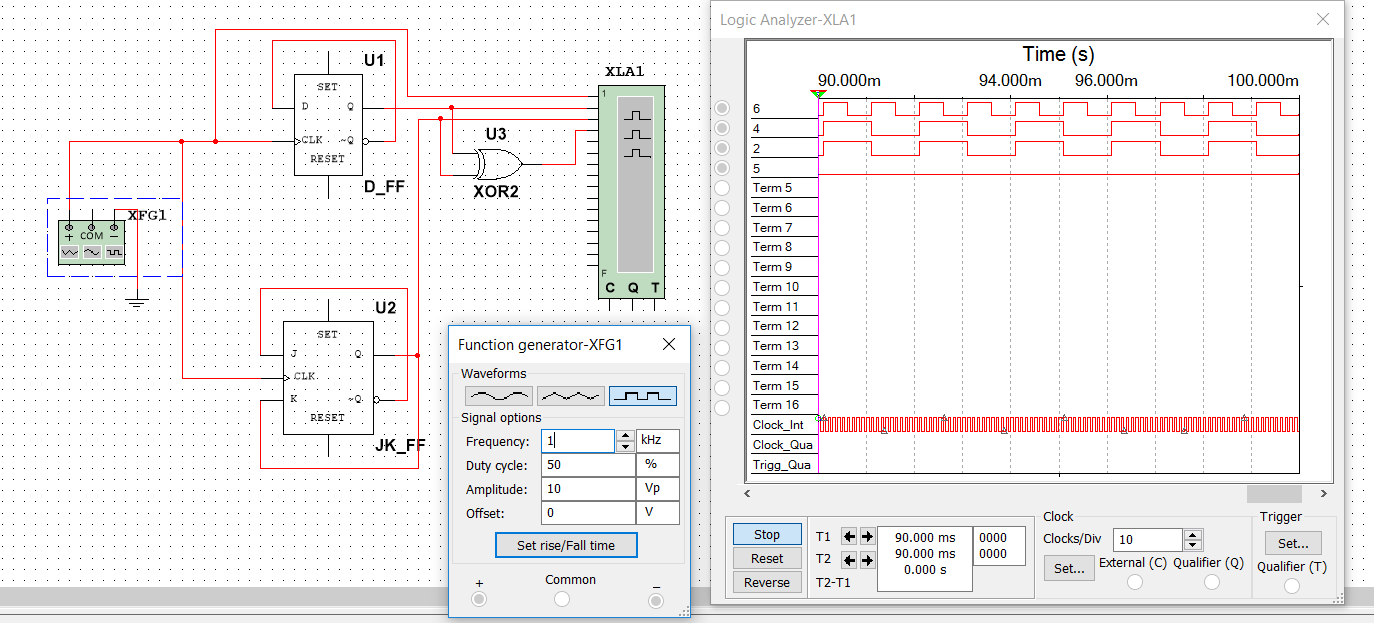
\includegraphics[width=\textwidth]{img/4a}
\end{figure}

\subsection{Przerzutnik D}
\begin{figure}[H]
\centering
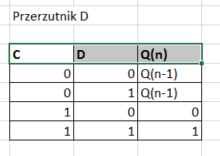
\includegraphics{img/4a_table_d}
\end{figure}
Chcemy, aby wartość logiczna Q zmieniała się na przeciwną niż dotychczasowa tylko, gdy sygnał zegara jest wzrastający.

Właściwości przerzutnika D, pozwalają na uzyskanie zmiany wartości wyjścia na wartość podaną na wejście D tylko, gdy sygnał zegara jest wzrastający. Jak jednak uzyskać zmianę sygnału na wręcz przeciwny? 
Na wejście D trzeba podać zanegowanie obecnej wartości sygnału Q - czyli -Q.

\subsection{Przerzutnik JK}

\begin{figure}[H]
\centering
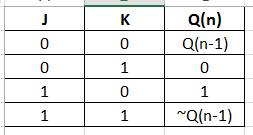
\includegraphics{img/4a_table_jk}
\end{figure}

Wyjście przerzutnika JK zmienia swój stan tylko wtedy, gdy sygnał zegara jest wzrastający. Ponadto, sygnał wyjściowy jest ustawiany zawsze na wartość wejścia J, gdy na wejścia J i K są podane przeciwne sygnały. 

W związku z tym wystarczy na wejście K podać sygnał wyjściowy (Q), a na wejście J - zanegowany sygnał wyjściowy (-Q). Mamy wtedy gwarancję, że sygnał przerzutnika zmieni się na wartość przeciwną do dotychczasowej.

\section{Czterobitowy licznik asynchroniczny}

\section{Licznik mod 8}

\section{Licznik mod 6}




\end{document}
